
\documentclass[11pt]{article}
%%%%%%%%%%%%%%%%%%%%%%%%%%%%%%%%%%%%%%%%%%%%%%%%%%%%%%%%%%%%%%%%%%%%%%%%%%%%%%%%%%%%%%%%%%%%%%%%%%%%%%%%%%%%%%%%%%%%%%%%%%%%%%%%%%%%%%%%%%%%%%%%%%%%%%%%%%%%%%%%%%%%%%%%%%%%%%%%%%%%%%%%%%%%%%%%%%%%%%%%%%%%%%%%%%%%%%%%%%%%%%%%%%%%%%%%%%%%%%%%%%%%%%%%%%%%
\usepackage{geometry}
\usepackage{setspace}

%TCIDATA{OutputFilter=LATEX.DLL}
%TCIDATA{Version=5.50.0.2960}
%TCIDATA{<META NAME="SaveForMode" CONTENT="1">}
%TCIDATA{BibliographyScheme=Manual}
%TCIDATA{Created=Tuesday, April 19, 2011 13:53:53}
%TCIDATA{LastRevised=Tuesday, April 30, 2013 22:43:51}
%TCIDATA{<META NAME="GraphicsSave" CONTENT="32">}
%TCIDATA{<META NAME="DocumentShell" CONTENT="Standard LaTeX\Blank - Standard LaTeX Article">}
%TCIDATA{CSTFile=40 LaTeX article.cst}

\newtheorem{theorem}{Theorem}
\newtheorem{acknowledgement}[theorem]{Acknowledgement}
\newtheorem{algorithm}[theorem]{Algorithm}
\newtheorem{axiom}[theorem]{Axiom}
\newtheorem{case}[theorem]{Case}
\newtheorem{claim}[theorem]{Claim}
\newtheorem{conclusion}[theorem]{Conclusion}
\newtheorem{condition}[theorem]{Condition}
\newtheorem{conjecture}[theorem]{Conjecture}
\newtheorem{corollary}[theorem]{Corollary}
\newtheorem{criterion}[theorem]{Criterion}
\newtheorem{definition}[theorem]{Definition}
\newtheorem{example}[theorem]{Example}
\newtheorem{exercise}[theorem]{Exercise}
\newtheorem{lemma}[theorem]{Lemma}
\newtheorem{notation}[theorem]{Notation}
\newtheorem{problem}[theorem]{Problem}
\newtheorem{proposition}[theorem]{Proposition}
\newtheorem{remark}[theorem]{Remark}
\newtheorem{solution}[theorem]{Solution}
\newtheorem{summary}[theorem]{Summary}
\newenvironment{proof}[1][Proof]{\noindent\textbf{#1.} }{\ \rule{0.5em}{0.5em}}
%\input{tcilatex}
\setlength{\parindent}{0in}
\renewcommand{\arraystretch}{.95}
\geometry{left=.8 in,right=.8 in,top=.8 in,bottom=.8 in}

\usepackage{graphicx}
\usepackage{dsfont}
\usepackage{amsmath}
\usepackage{epsfig}
\usepackage{epstopdf}
\usepackage{subfigure}
\usepackage{array}
\newcolumntype{L}[1]{>{\raggedright\let\newline\\\arraybackslash\hspace{0pt}}m{#1}}
\newcolumntype{C}[1]{>{\centering\let\newline\\\arraybackslash\hspace{0pt}}m{#1}}
\newcolumntype{R}[1]{>{\raggedleft\let\newline\\\arraybackslash\hspace{0pt}}m{#1}}
\DeclareMathOperator*{\argmax}{argmax}
\DeclareMathOperator*{\argmin}{argmin}
\usepackage{listings}



\begin{document}

\textbf{Isolating variable cost components}


There's no point in re-inventing the wheel. But the wheel we have (E3 ACC) is not perfectly suited for our application. The E3 ACC is designed to estimate cost avoided by a DER investment that reduces demand over a longer, forward-looking time frame. Their focus is on estimating costs avoided by future demand reductions We are looking retrospectively and asking what was the variable cost incurred by realized demand.  


\bigskip

The following tries to unpack what the ACC does vis a vis the cost components we want to isolate. I also relate E3 methods to methods used in IOU general rate cases (GRCs).

\bigskip

 The figure below shows the relative importance of the key cost components (using 2020 ACC).

\bigskip


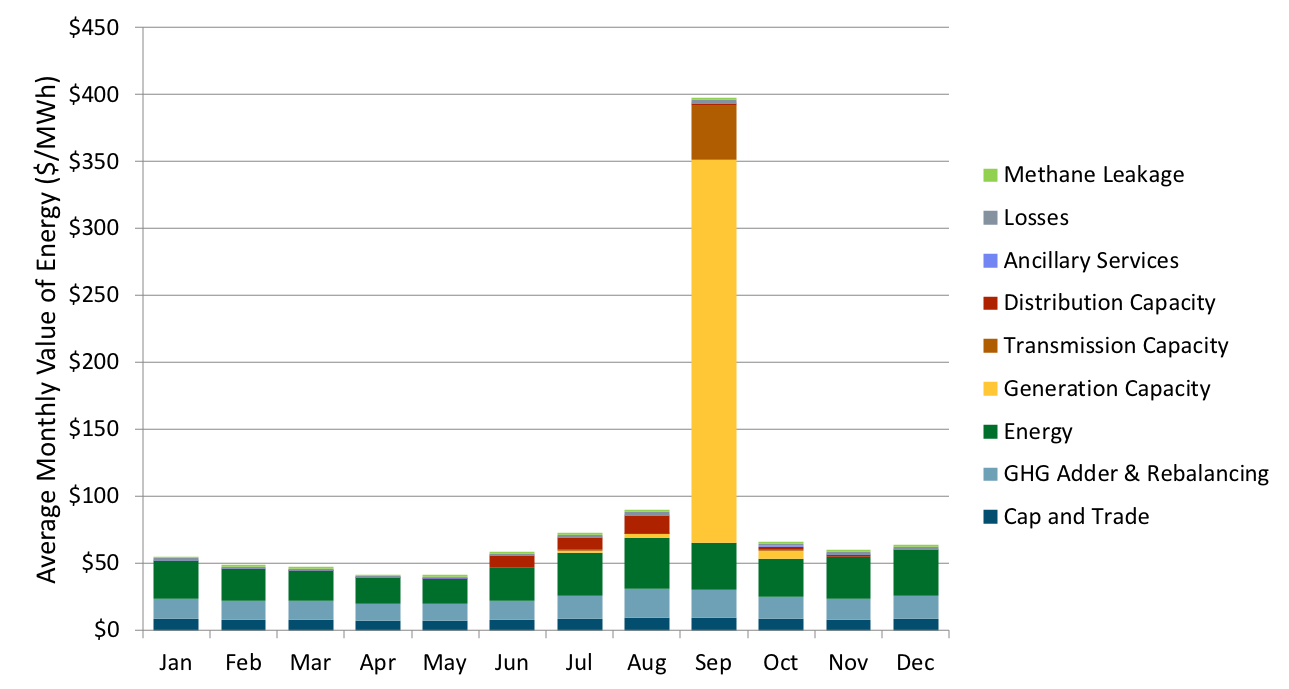
\includegraphics[scale=0.7]{ACC2020.png}

\section{Definitions}

The marginal cost associated with an increase in customer electricity usage are comprised of multiple components:

\subsection{Marginal Energy Cost (MEC = green)}

\begin{itemize}


\item The MEC is the cost of procuring electricity to meet one additional megawatt-hour (MWh) of load, measured in cents per kilowatt-hour. 

\item Because the IOUs meet residual needs by purchasing power in the CAISO day-ahead market, long-term ISO wholesale energy price forecast could be used to estimate the MEC.

\item In recent years, E3 and some IOUs have started to use production simulation models (PLEXOS, SERVM) versus ISO forecast prices to estimate this component. 

\item Key methodological differences pertain to forecasting far into the future. Because we will be using one year ahead forecasts (correct?) I think we need to be less concerned with the assumptions behind this component.

\item One issue: GHG costs. IOUs versus E3 quite different.

\end{itemize}


\subsection{GHG component (blue)}

\begin{itemize}



\subsection{Marginal Generation Capacity Costs (MGCC) yellow}

\begin{itemize}

\item The MGCC captures the fixed cost of procuring and operating generation capacity to meet one additional megawatt of peak load. These are measured in terms of  dollars per kilowatt-year. 

\item In GRC cases, a Peak Capacity Allocation Factor (PCAF) is used to allocate \$/kW-year to specific hours.

\item One notable difference. In some GRCs, utilities focus on avoided fixed operating costs. E3 emphasizes avoided investment costs in new capacity (CCGT in past years, storage in 2020)


\end{itemize}



\subsection{Marginal Transmission Capacity Costs (MTCC) }

\begin{itemize}

\item Deferrable transmission projects are `demand-related' marginal  transmission investments.

\item On a regular basis, IOUs coordinate with the California Independent System Operator (CAISO) to plan transmission expansion upgrades (5 to 10 year time frame). If a given facility loading is reduced considerably prior to the implementation date, due to demand forecasts, then the implementation date of a planned transmission project may be deferred. 

\item If a project is deemed to be `deferrable', this means that the  project is driven by demand, and not by regulatory, safety, contractual, efficiency or other reasons. 

\item Marginal transmission capacity costs are based on these deferrable transmission projects.

%\item Although IOU transmission rates are regulated by FERC,  MTCC values are required for purposes other than determining revenue requirements for rate setting. One example:  MTCC values are used in marginal cost price floor calculations.

\item IOU-specific forward-looking MTCCs are estimated using the Discounted Total Investment Method (DTIM).

\begin{enumerate}

\item Calculate the marginal investment per megawatt (MW) as the present value of deferrable investments divided by the present value of forecast load growth. The result is the marginal investment per MW. 

\item Calculate an annualized marginal cost in dollars per MW per year using a Real Economic Carrying Charge (RECC) factor. The resulting marginal cost reflects the annualized cost of investment as well as other capital costs and annual expenses associated with adding capacity to the transmission system. 

\end{enumerate}


\item Note that the RECC takes the investment cost and reshapes them to reflect a stream of costs that increases with inflation and has the same present value as the revenue requirements. Inputs to a RECC: the capital structure and cost of capital, a discount rate, income tax parameters, book depreciable life and costs of
property taxes and insurance. 


\item \textbf{Point of confusion:} The PG&E GRC  estimates   a single demand-related  MTCC in dollars per kW per year of  of \$11.48.  Shouldn't this vary by location?  

\end{itemize}


\subsection{Marginal Distribution Capacity Costs (MDCC)}
\begin{itemize}

\item MDCC values are used for marginal cost revenue calculations and rate design, avoided cost modeling, among other things. 


\item PG&E’s distribution system is defined as facilities operated at voltages less than 50 kilovolts (kV). The system is further divided into primary distribution system (>4V); and  the secondary distribution system. 

\item A detailed planning process uses uses peak load data and load growth forecasts to evaluate whether existing substation and feeder capacity is sufficient so that equipment is not overloaded and so that  service-operating parameters (e.g., voltage limits and adequate reliability levels) are maintained under both normal, and emergency operating conditions.

\item As a general rule, the costs of operating, maintaining and replacing distribution equipment, once installed, are independent of usage. Such costs associated with existing distribution equipment are properly considered fixed
costs and excluded from marginal cost calculations.

\item However, there are two types of investments that are made to meet demand growth: (1) Distribution reinforcement investments provide capacity  to meet demand growth on the existing system and (2) distribution investments for primary line extensions provide access and the associated capacity for new demand due to the addition of new customers. 

\item MDCC are calculated using the DTIM.  Same process as above:

\begin{enumerate} 

\item Calculate the present value for a stream of capacity-related  investments and divide that present value amount by the present value of the corresponding capacity growth (in kW): the result is a marginal investment cost for a kW change in capacity.  The forecasted investment for large projects and  forecasted capacity growth  are provided by  PG&E’s Distribution System Planning Department. These large  projects generally cause marginal cost “lumpiness” over both geographic and time dimensions.
 
\item The incremental investment costs per unit of capacity are converted to an annualized marginal cost per unit of capacity by applying a Real Economic Carrying Charge (RECC) factor and  appropriate loadings. 

\end{enumerate}

\item The Commission has indicated that marginal costs should “reflect geographic differences where significant.” PG&E
has a wide variation in the marginal cost of distribution capacity among the more than 240 DPAs that comprise its electric system. Accordingly, PG&E  estimates marginal
costs by DPA, and then aggregates those costs into PG&E’s operating divisions.

\item PG&E estimates MDCC values for three subcomponents: (1) marginal primary distribution capacity costs;  (2) marginal primary distribution capacity costs for new business; and (3) marginal secondary distribution capacity costs. 

\item Primary distribution marginal costs are shown in dollars per PCAF-kilowatt (kW) per year and primary distribution for new  business and secondary distribution marginal costs are shown in dollars per FLT-kW per year.  

\item To match these marginal costs with kWh, we need to define the distribution Peak Capacity Allocation Factors (PCAF).

\end{itemize}


\section{E3 ACC}

\subsection{MEC}

\begin{itemize}

\item  In past GRC filings,  PG&E forecasts hourly prices  over a 6 year time horizon based on historical day-ahead prices. The MEC for each of PG&E’s six TOU periods is estimated as the average of the hourly electricity price forecasts weighted by the hourly 2014 PG&E system loads (time-shifted so that weekends line up between hourly prices and hourly loads).

\item In contrast, SCE uses an internal PLEXOS production simulation model to forecast ISO market clearing prices over a 3 year period for GRC filing.

\item Prior to 2020, E3 near-term energy costs were based on on-peak and off-peak market forecasts when available.
For the periods farther into the future, they interpolate between the latest available forward price and the long-run energy market price (set so that a CCGT energy market revenues \textit{plus the capacity market payments} equals fixed and variable cost plus carbon costs).

%\item \textbf{Confusion \#1} I am confused about the long  interactions between simulated long run energy price and assumptions about capacity prices? And I am confused how short and long term prices are weighted in their MEC measures.

%\item Hourly shaping: They convert annual energy avoided cost to hourly values using 8760 `market shapes' derived from LMPs at NP15 and SP15. 


\item  The 2020 E3 ACC has moved to using production simulation do develop energy values for the ACC. Use a  production simulation model (SERVM).   Market prices reported directly from SERVM include the effects of carbon pricing from the cap and trade market. In post-processing the SERVM prices, the cap and trade value is backed out to provide an hourly energy only value for use in the ACC. The remaining energy value includes only fuel costs and power plant operating costs.

\end{itemize}

\textbf{Comment}: Differences in methods seem most significant far into the future. We should be setting the time frame to one year, correct?

\textbf{Question}: One methodological difference across sources/years: treatment of GHG permit value. How do we want to deal with this component?


\subsection{GHG costs}

\begin{itemize}

\item In early ACC calculations, the GHG costs were based on changes in GHG output of the marginal generating unit in each hour of the year (i.e. the marginal emissions rate). 

\item Pre-2020 E3  GHG values represented by the sum of the monetized GHG permit cost embedded in energy prices and the non-monetized GHG value beyond the permit price.

\item Recent methodological changes (2020) respond to the fact that a DER investment will impact future emissions as the system is rebalanced to reflect new levels of consumption and emissions. This rebalancing issue has become more of an issue with the increased focus on electrification, rebalancing of emissions to meet annual targets could be significant.

\end{itemize}

\texbf{Comment} Playing around with the 2020 calculator, rebalancing has a non-negligible impact on a one year forecast. Figure below turns off `rebalancing' *Ask E3 about this.*



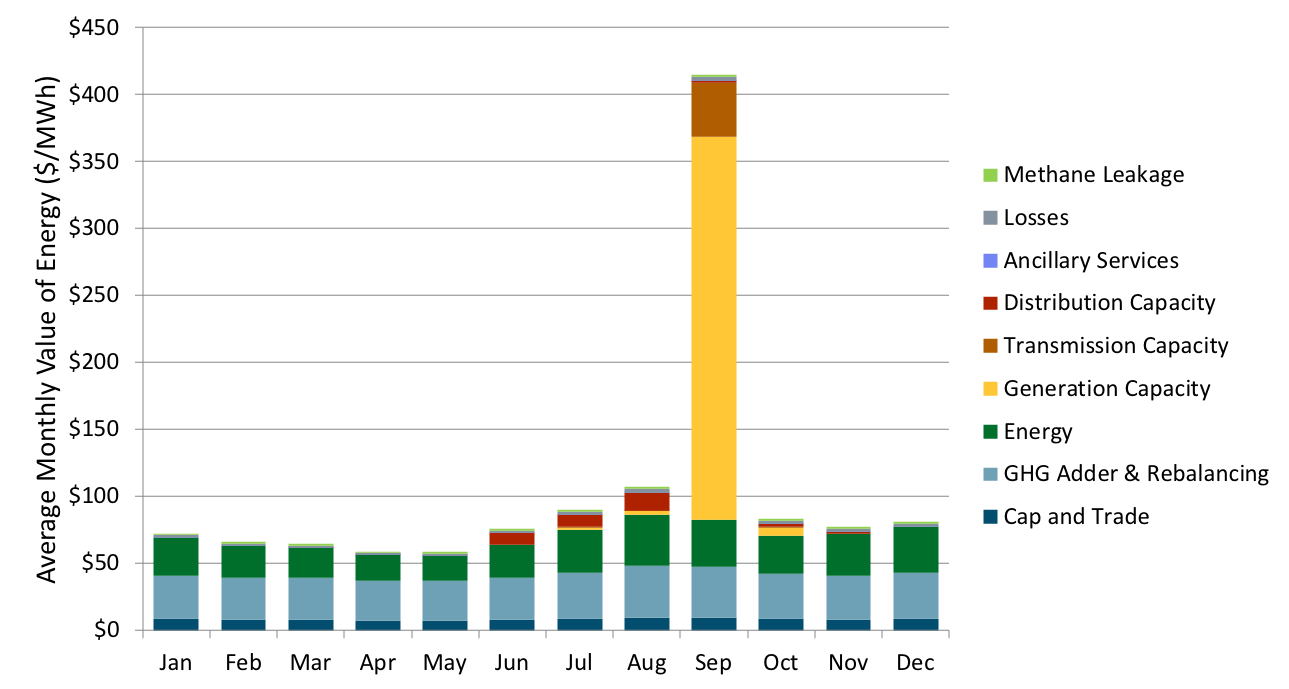
\includegraphics[scale=0.7]{ACC2020nobalance.png}

\textbf{Question} How do we want to deal w GHG costs for our purposes?

\subsection{MGCC}

\begin{itemize}

\item For example, in the 2016 GRC, PG&E estimated the short-run cost of capacity as the going-forward fixed cost of the existing generation resource net of energy gross margins it earns from the spot energy market over the period  2017-2022.  They assumed an existing combined cycle gas turbine (CCGT) plant as the marginal unit. The going-forward fixed cost consists of fixed O&M, insurance and property tax. Insurance and property tax are estimated based on the capital costs.  Notably, this is not a `growth-driven' cost.


\item  PG&E estimated net costs of capacity:  \$30.23/kW-year, \$29.62/kW-yr, \$28.53/kW-yr, \$27.63/kW-yr, \$27.70/kW-yr and \$27.42/kW-yr for 2017 through 2022, respectively. This represents the cost of an existing CCGT’s fixed costs above and beyond what it could earn in the energy market


\item To calculate levelized MGCC, PG&E first calculated a Net Present Value (NPV) sum of the six years of MGCCs and then converted this NPV to a levelized value using the same discount rate. PG&E used its after-tax Weighted Average Cost of Capital (WACC) of 7.0 percent. The resulting levelized MGCC is \$28.64/kW-year. This is much lower than the E3 ACC .... I think because it is not the cost of building new capacity to meet increasing peak, it's the fixed cost of meeting current peak. 

\item In a final step, a weighted portion of demand related costs is assigned to every hour in excess of 80\% of peak demand.  This PCAF calibration proceeds in three steps:

\begin{enumerate}

\item Identify the PCAF hours: Generation PCAF hours are defined as hours during which the total system load is above 80 percent of the system maximum load during the calendar year. 

\item For each identified PCAF hour, the corresponding PCAF weight is constructed such that the peak hour has an allocation that is 20 times the allocation for the hours at 81\% of peak demand and twice the allocation of an hour at 90\% of peak demand.

\item Using customer class net metered loads, calculate
PCAF-weighted loads for each customer class.

\end{enumerate}
\end{itemize}


\textbf{Stupid question}:  If we allocate MGCC costs to *hours*  using this PCAF factor, does this guarantee that revenues earned over and above variable costs equal the levelized MGCC to be recovered in expectation? 


\item Prior to 2020, E3 estimates the levelized capital cost of a new CCGT  unit less the margin the plant would earn on the energy and ancillary service markets (including carbon costs)

\item The 2020 ACC calculates the Net Cost of New Entry (CONE) of a new battery storage resource instead of a gas combustion turbine.

\item Start with the capital cost and subtract simulated market revenues from energy and AS markets.

\item Capacity value is increased to account for planning reserve margins.

\item To allocate these capacity values across hours of the year, they use the E3 RECAP model ``which determines the expected unserved energy for each month/hour/day.'' This assumes there will be a need for new capacity going forward.

\item \textbf{Point of confusion number 1:} Whereas IOUs seem to focus on going forward fixed operating costs, E3 focusing on new investment costs. E3 2018 MGCC estimates much higher than PG&E estimates.

\item \textbf{Point of confusion number 1:} Minor issue- E3 seems to use a different approach to allocate capacity costs to hours.

\end{itemize}

\subsection{MDCC}


\item The 2017 PG&E rate filing lists MDCC results for each division (Table 6-1). This is similar to- but different from- the numbers used by the E3 ACC.  They use 2014 GRC numbers (Table 4)  which are mostly (but not all) higher.

\item Similarly, the distribution costs assumed by the ACC are taken from a 2015 GRC and are higher than those reported in the 2018 GRC.

\item The ACC allocates these T&D capacity costs to hours using a regression model that predicts hourly distribution demand as a function of temperature, HDD, CDD, hour and month FE. They then subtract off forecast PV penetration.

\item They simulate distribution loads using 2017 weather data for each climate zone.   They then compare these simulated hourly load against these climate zone specific thresholds (defined as the area maximum demand less one standard deviation??) : $(Load[a,h]-Threshold[a]$.

\item They normalize these by the sum of all positive differences to estimate peak capacity allocation factors (PCAF) for each climate zone and hour.  Intuitively, if  we sum across *all* kWh charged this capacity cost (not just residential), should we recover the reported annualized marginal cost per unit of capacity?  If yes, not clear how this approach delivers this result.

\end{itemize}
\end{document}


